\documentclass[12pt]{article}

\usepackage{fontspec}
\usepackage{polyglossia}
\setdefaultlanguage{russian}
\setotherlanguage{english}

\setmainfont{TeX Gyre Pagella}
\setsansfont{TeX Gyre Adventor}

\newfontfamily\cyrillicfont{Palatino Linotype}
\newfontfamily\cyrillicfontsf{Arial}
\newfontfamily\cyrillicfonttt{Courier New}

\usepackage{geometry}
\usepackage{sectsty} % change the appearance of \section
\usepackage{fontawesome5}
\usepackage{xcolor}
\usepackage{graphicx}
\usepackage{tikz}
\usepackage{xstring}
\usepackage{tcolorbox}
\usepackage{lipsum}
\usepackage{enumitem}
\usepackage{blindtext}
\usepackage{hyperref}
\usepackage[none]{hyphenat}
\usepackage{unicode-math}
\emergencystretch=3em
\geometry{
  a4paper,
  left=20mm,
  right=20mm,
  bottom=10mm,
  top=15mm
}
  
\pagestyle{empty}

\sectionfont{
    \sffamily
    \sectionrule{0pt}{0pt}{-8pt}{1.5pt}
}

%%%%%%%%%%%%% Macros %%%%%%%%%%%%%

%%%%%%%%%%%%% Colors %%%%%%%%%%%%%

\definecolor{blueSky}{RGB}{49, 120, 198}
\definecolor{orangeFruit}{RGB}{224, 128, 44}
\definecolor{redBlood}{RGB}{188, 20, 20}
\definecolor{grayShy}{RGB}{153, 150, 142}
\definecolor{Blue}{RGB}{40, 150, 180}

\newcommand{\mainColor}{Blue}

%%%%%%%%%%%%% Spaces %%%%%%%%%%%%%

\newlength{\spacebox}
\settowidth{\spacebox}{123456789}

\newcommand{\xhspace}{\hspace*{0.1em}}
\newcommand{\shspace}{\hspace*{0.5em}}
\newcommand{\mhspace}{\hspace*{1em}}

\newcommand{\negxhspace}{\hspace*{-0.2em}}
\newcommand{\negshspace}{\hspace*{-0.5em}}
\newcommand{\negmhspace}{\hspace*{-1em}}
\newcommand{\neghhspace}{\hspace*{-1.5em}}

\newcommand{\negxvspace}{\vspace*{-0.2em}}
\newcommand{\negsvspace}{\vspace*{-0.5em}}
\newcommand{\negmvspace}{\vspace*{-1em}}
\newcommand{\neghvspace}{\vspace*{-1.5em}}

\newcommand{\svspace}{\vspace*{0.5em}}
\newcommand{\mvspace}{\vspace*{1em}}

\newcommand{\boxAwesome}[1]{
   \makebox[1.50em][c]{
      #1
   }
}

\newcommand{\job}[1]{
  \large
  \color{grayShy}
  \begin{center} #1 \end{center}\par \mvspace
}

\newcommand{\name}[3]{
    \begin{center}
        \begin{tikzpicture}
            \clip (0,0)  circle (2.2cm) ;
            \node[anchor=center] at (0, 0) {
                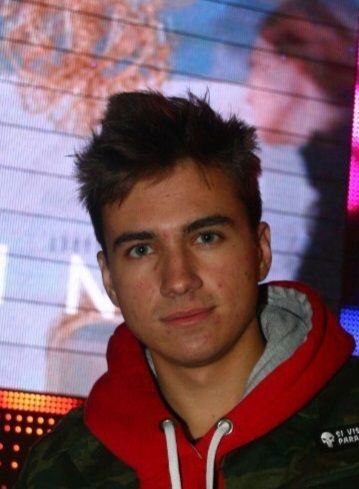
\includegraphics[scale=0.4]{img/avatar.jpg}
            };
        \end{tikzpicture}
    \end{center}
    \hfill
    \Huge
    \sffamily 
    \begin{center} \color{\mainColor} \textbf{\MakeUppercase{#1}} \color{black} \textbf{#2} \end{center}\par
    \negxvspace
    \job{#3}
    \normalsize\normalfont
    \color{black}
}

\newcommand{\cvsection}[2]{
    \section*{
        \color{\mainColor} \boxAwesome{#1} \negshspace #2
    }
}

\newcommand{\cvsubsection}[2]{
    \subsection*{
        \boxAwesome{#1} #2
    }
}

\newcommand{\info}[2]{
  \noindent\hangindent=2em\hangafter=0
  \boxAwesome{#1}
  #2 \par
  \svspace
}

\usepackage{xurl}

\newcommand{\site}[1]{{\normalfont\sffamily\mdseries\small\color{grayShy}\url{#1}}}

\newcommand{\simpleSkill}[1]{
    \noindent\hangindent=1.5em\hangafter=0
    \faAngleRight
    \shspace
    #1
    \svspace
    \par
}

\newcommand{\doubleSkill}[3]{
    \noindent\hangindent=1.5em\hangafter=0
    \parbox{30\spacebox} {
        \faAngleRight
        \boxAwesome{#1} \textbf{#2}
        \svspace
    } \svspace \texttt{#3} \par
    \vspace*{0.25em}
}

\newcommand{\work}[4]{
    \noindent \textbf{#1}
    \hfill
    \framebox{
      \parbox{8em}{
      \centering\textbf{#2}
    }} \par
    \noindent {\normalsize\color{grayShy}#3} \color{black} \par
    \noindent\hangindent=1.5em\hangafter=0 #4 \par
    \mvspace
    \normalsize \par
}
\newcommand{\workSubrole}[3]{
    \noindent {\normalsize\textbf{#1}}
    \hfill
    \framebox{
      \parbox{8em}{
      \centering\textbf{#2}
    }} \par
    \noindent\hangindent=1.5em\hangafter=0 #3 \par
    \svspace
}

\newcommand{\education}[3]{
   \noindent \textbf{#1}
   \hfill
   \framebox{
      \parbox{8em}{
      \centering\textbf{#2}
    }} \par
    \noindent \color{grayShy} \textsc{\MakeLowercase{#3}} \color{black} \par
    \mvspace
    \normalsize \par
}

\newcommand{\hobby}[2]{
    \noindent\hangindent=1.5em\hangafter=0
    \faAngleRight
    \shspace
    \boxAwesome{#1} #2
    \svspace
    \par
}

\newcommand{\projectTitle}[1]{
    \noindent\hangindent=1.5em\hangafter=0
    \faAngleRight
    \shspace
    {\normalsize\textbf{#1}} \par
    \negxvspace
}

\newcommand{\projectDesc}[1]{
    {\small\linespread{1.05}\selectfont #1 \par}
    \negxvspace
}

\newcommand{\projectTools}[1]{
    \svspace
    {\small \textit{\textbf{Инструменты:}} #1 \par}
    \mvspace
    \svspace
}


%%%%%%%%%%%%% Your CV below %%%%%%%%%%%%%

\begin{document}
    \name{Николай Тулупов}{}{студент 4 курса, встраиваемые системы и радиотехника}

    \info{\faEnvelopeOpen}{\texttt {tulupov.nd@phystech.edu}}
    \info{\faGithub}{\href{https://github.com/oncominglane}{\texttt{oncominglane}}}
    \info{\faVk}{\href{https://vk.com/oncoming_lane}{\texttt{vk.com/oncoming\_lane}}}
    \info{\faTelegram}{\href{https://t.me/oncoming_lane}{\texttt{t.me/oncoming\_lane}}}
        
    \negsvspace
    \cvsection{\faDna}{Ключевые навыки}
    \svspace
    \cvsubsection{\faLaptopCode}{Технические навыки}
    \svspace
    
    \doubleSkill{\faCode}{Языки программирования}{C/C++ \textbullet{} Python \textbullet{} x86-64 assembly}
    
    \doubleSkill{\faTools}{Инструменты}{MATLAB \textbullet{} Motor-CAD \textbullet{} CMake \textbullet{} Git \textbullet{} Xilinx ISE \textbullet{} EasyEDA \textbullet{} LaTeX}
    
    \doubleSkill{\faDesktop}{Устройства}{Arduino \textbullet{} STM32 \textbullet{} AT32 \textbullet{} Raspberry Pi \textbullet{} NAPI}

    \doubleSkill{\faMicrochip}{Встраиваемые системы и интерфейсы}{UART \textbullet{} SPI \textbullet{} I2C \textbullet{} CAN \textbullet{} GPIO \textbullet{} RS232 \textbullet{} ALSA}
    
    \doubleSkill{\faLinux}{ОС}{Linux (Ubuntu, Armbian) \textbullet{} Windows}
    
    \doubleSkill{\faHammer}{Практические навыки}{Пайка \textbullet{} Механическая обработка \textbullet{} 3D-печать \textbullet{} Лазерная резка}
   
    \negsvspace
    \cvsubsection{\faHandsHelping}{Ключевые компетенции}
    \svspace

    \simpleSkill{Решение сложных инженерных задач}
    \simpleSkill{Быстрая обучаемость и адаптивность}
    \simpleSkill{Техническая коммуникация}
    \simpleSkill{Системное мышление}
    

    \cvsection{\faGraduationCap}{Образование}
    \svspace
    
    \education{Московский физико-технический институт}{2022 - 2026}{Факультет радиотехники и компьютерных технологий}

    \cvsection{\faDesktop}{Опыт работы}
\svspace

\work{ПромСвязьРадио ООО  \href{http://prsvradio.ru/}{\site{prsvradio.ru}}}{02.2024 \textendash\ н.в.}{Помощник инженера}{Диагностика радиооборудования, ведение технической документации и координация инженерных задач.}

\noindent \textbf{АмперМагнит АО  \href{https://ampere.amtc.ru/ru/}{\site{ampere.amtc.ru/ru}}} \par
\noindent {\normalsize\color{grayShy}Стажёр-инженер} \color{black} \par
\workSubrole{Группа разработки контроллеров}{09.2024 \textendash\ 03.2025}{Разработка логики прошивки контроллера AC зарядной станции в соответствии со стандартом GB/T 18487.}
\workSubrole{Группа разработки ИИ}{03.2025 \textendash\ 02.2026}{Оптимизация систем управления электроприводами и разработка встроенного ПО силовых инверторов.}
\mvspace

\work{Московский физико-технический институт \\ Лаборатория робототехники и электромобильности \\ \href{https://mipt.ru/education/basic-departments/kafedra-elektromobilnosti-i-magnitnykh-sistem}{\site{mipt.ru/.../kafedra-elektromobilnosti...}}}{02.2026 \textendash\ н.в.}{Техник-исследователь}{Оптимизация систем управления электроприводами и подготовка научных публикаций.}


  \neghvspace
\cvsection{\faBook}{Проекты}
\svspace

\projectTitle{Система удалённого управления радиостанцией Motorola XTL2500}
\projectDesc{Спроектирована и реализована распределённая клиент-серверная система на базе одноплатных компьютеров (NaPi) для удалённого управления радиостанцией. Реализованы двунаправленная передача аудио в реальном времени, обработка управляющих команд и взаимодействие по протоколам SB9600/SBEP с разбором кадров и декодированием данных дисплея. Выполнена интеграция интерфейсов ADC/DAC и UART/SPI/I2C. Ведётся разработка печатной платы, корпуса и технической документации.}
\projectTools{C/C++, Linux, CMake, NaPi/Raspberry Pi, Ethernet, UART/SPI/I2C, разработка печатных плат}

\projectTitle{Оптимизация управления приводом IPMSM и исследование методов обучения с подкреплением}
\projectDesc{Разработаны и верифицированы методы оптимизации управления приводом IPMSM, включая новый подход к оценке электромагнитного момента контроллером инвертора, реализацию прошивки инвертора на базе AT32 и проведение экспериментальных исследований на испытательном стенде. Проведено исследование методов обучения с подкреплением для задач управления приводом в среде моделирования.}
\projectTools{Python, C/C++, Motor-CAD, MATLAB/Simulink, PyTorch, AT32, встроенное ПО}

\projectTitle{StandControl: система управления инвертором по CAN}
\projectDesc{Разработана клиент-серверная система управления силовым инвертором по CAN-шине. Реализован графический интерфейс пользователя для управления режимами работы (момент, скорость, ток), визуализации телеметрии, ведения логирования и обработки ошибок. Реализован обмен CAN-сообщениями и сетевое взаимодействие с инвертором. Программный продукт зарегистрирован как ПО.}
\projectTools{C/C++, Python, CMake, CAN (PCAN), TCP/IP, DBC}

\neghvspace
\cvsection{\faBookOpen}{Публикации и конференции}
\svspace

\simpleSkill{\textbf{Экспериментальная идентификация и реализация компактной аналитической модели момента для управления приводом IPMSM} \\
Статья на рецензировании в \textit{eTransportation (Q1)}}

\simpleSkill{\textbf{III конференция "Технологии ИИ в науке и образовании"}, МГУ, декабрь 2025 \\
Лучший доклад (секция точных и инженерных наук), тезисы опубликованы в сборнике}

\simpleSkill{\textbf{XII международная конференция "Engineering \& Telecommunications (En\&T-2025)"}, МФТИ, ноябрь 2025 \\
Тезисы опубликованы в сборнике}

\simpleSkill{\textbf{68-я Всероссийская научная конференция МФТИ}, МФТИ, апрель 2025 \\
Доклад принят к представлению}

\simpleSkill{\textbf{27-я Международная конференция молодых специалистов в области электронных приборов и материалов (IEEE EDM)}, Алтай, июль 2026 \\
Работа на рецензировании}

    \neghvspace
    \svspace
    \cvsection{\faPuzzlePiece}{Хобби и интересы}
    \svspace

    \hobby{\faTv}{Радиотехника}
    \hobby{\faGuitar}{Игра на гитаре}
    \hobby{\faCar}{Автомобили}


\end{document}